\subsection{Round 1 Problems}

Solutions can be found in Section~\ref{S::2024-J-1}.

\mcq

\begin{enumerate}
    \hyperrefitem[Q::2024-J-1-1] If $x^2 + 4x + 16 = 0$, what is the value of $x^3$?
    \begin{tasks}(5)
        \task 4
        \task 8
        \task 16
        \task 64
        \task 128
    \end{tasks}
    \hyperrefitem[Q::2024-J-1-2] Let $a$ be a real number that satisfies $-1 < a < 0$. Which of the following is true?
    \begin{tasks}(5)
        \task! $\pi^a < \frac1\pi < (\frac1\pi)^a$
        \task! $\pi^a < (\frac1\pi)^a < \frac1\pi$
        \task! $\frac1\pi < (\frac1\pi)^a < \pi^a$
        \task! $\frac1\pi < \pi^a < (\frac1\pi)^a$
        \task! $(\frac1\pi)^a < \pi^a < \frac1\pi$
    \end{tasks}
    \hyperrefitem[Q::2024-J-1-3] How many non-congruent triangles are there whose sides have integer lengths and the longest side has length 10 units?
    \begin{tasks}(5)
        \task 25
        \task 30
        \task 35
        \task 40
        \task 45
    \end{tasks}
    \hyperrefitem[Q::2024-J-1-4] In the diagram below, the points $B$ and $E$ lie on $AF$ and $DF$ respectively, and $AE$ and $BD$ intersect at $C$. If $AB = AC$, $BD = BF$ and $EA = EF$, find $\angle BAC$.
    \begin{center}
        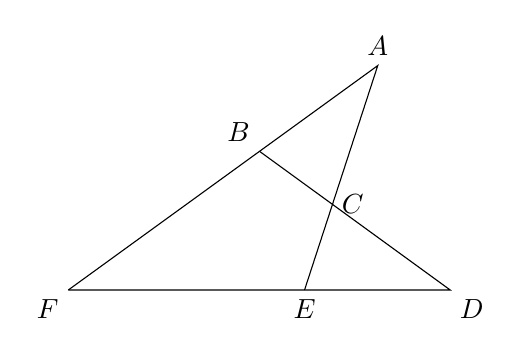
\begin{tikzpicture}
            \coordinate[label=above:$A$] (A) at (3.93, 2.85);
            \coordinate[label=above left:$B$] (B) at (2.43, 1.76);
            \coordinate[label=right:$C$] (C) at (3.35, 1.09);
            \coordinate[label=below right:$D$] (D) at (4.85, 0);
            \coordinate[label=below:$E$] (E) at (3, 0);
            \coordinate[label=below left:$F$] (F) at (0, 0);
    
            \draw (F) -- (A) -- (E);
            \draw (B) -- (D) -- (F);
        \end{tikzpicture}
    \end{center}
    \begin{tasks}(5)
        \task $30\deg$
        \task $33\deg$
        \task $36\deg$
        \task $38\deg$
        \task $40\deg$
    \end{tasks}
    \hyperrefitem[Q::2024-J-1-5] Let $x$, $y$ and $z$ be real numbers such that $x \neq 0$, $y - z \neq 0$ and $z + x \neq 0$. If $\dfrac{2}{x} = \dfrac{4}{y - z} = \dfrac{5}{z + x}$, find the value of $\dfrac{7x-y}{y+2z}$.
    \begin{tasks}(5)
        \task $\dfrac{11}{17}$
        \task $-\dfrac{11}{17}$
        \task $\dfrac{7}{13}$
        \task $-\dfrac{7}{13}$
        \task 1
    \end{tasks}
\end{enumerate}

\clearpage
\sq

\begin{enumerate}
    \setcounter{enumi}{5}
    \hyperrefitem[Q::2024-J-1-6] Let $N$ be a 2-digit whole number. When 2692 is divided by $N$, the remainder is 13, and when 2978 is divided by $N$, the remainder is 14. Find the sum of all the possible values of $N$.
    \hyperrefitem[Q::2024-J-1-7] If $x$ is a positive integer such that $2^x + 2^{89} = 512^{10}$, find the value of $x$.
    \hyperrefitem[Q::2024-J-1-8] The diagram shows a right-angled triangle $ABC$. The sides $AC$ and $AB$ are in the ratio $3:5$. The point $D$ lies on $BC$ such that $AD$ is perpendicular to $BC$. Furthermore, $DB$ is 8 cm longer than $CD$. What is the length of $BC$ in cm?

    \begin{center}
        \begin{tikzpicture}[scale=0.4]
            \coordinate[label=below left:$A$] (A) at (0, 0);
            \coordinate[label=below right:$B$] (B) at (14.577, 0);
            \coordinate[label=above left:$C$] (C) at (0, 8.746);
            \coordinate[label=above right:$D$] (D) at (3.858, 6.43);

            \draw (A) -- (B) -- (C) -- (A) -- (D);

            \draw pic [draw, angle radius=2mm] {right angle = C--A--B};
            \fill (D) circle[radius=5pt];
        \end{tikzpicture}
    \end{center}
    \hyperrefitem[Q::2024-J-1-9] Let $n$ be a positive integer. Suppose that $a_1, a_2, a_3, \ldots$ is a sequence of numbers defined by \[a_1 = \sqrt{(n+3)(n-1) + 4}, \quad a_k = \sqrt{(n + 2k + 1)a_{k-1} + 4} \quad \text{for $k \geq 2$}.\] If $a_{100} = 2024$, find the value of $n$.
    \hyperrefitem[Q::2024-J-1-10] Let $N$ be the smallest positive integer such that the sum of its digits is 2024. What is the sum of the digits of the number $N + 2$.
    \hyperrefitem[Q::2024-J-1-11] If $a$ and $b$ are non-zero real numbers such that $\dfrac1b - \dfrac1a = 4$, find the value of $\dfrac{3a + 7ab - 3b}{a - 3ab - b}$.
    \hyperrefitem[Q::2024-J-1-12] If the 5-digit whole number $\ol{11ab6}$ is a perfect square, find the value of $a + b$.
    \hyperrefitem[Q::2024-J-1-13] Let $N = 1 \times 2 + 2 \times 3 + 3 \times 4 + \cdots + 30 \times 31$. Find the value of $N$.
    \hyperrefitem[Q::2024-J-1-14] Let $x$ and $y$ be non-zero real numbers where $x \neq y$. If $x^2 + \sqrt3 y = 4$ and $y^2 + \sqrt3 x = 4$, find the value of $\bp{\dfrac{y}{x}}^2 + \bp{\dfrac{x}{y}}^2$.
    \hyperrefitem[Q::2024-J-1-15] Find the sum of all 2-digit even numbers $N$ with the following property: $N$ is a multiple of the product of its two digits.
    \clearpage
    \hyperrefitem[Q::2024-J-1-16] In the diagram below, $AEB$ is an isosceles right-angled triangle and $ABG$ is a $30\deg$-$60\deg$-$90\deg$ right-angled triangle with $\angle GAB = 30\deg$. The sides $AG$ and $BE$ intersect at $H$. If the area of triangle $AHE$ is 50 cm$^2$, find the area of triangle $BGH$ in cm$^2$.
    
    \begin{center}
        \begin{tikzpicture}
            \coordinate[label=below left:$A$] (A) at (-4, 0);
            \coordinate[label=below right:$B$] (B) at (4, 0);
            \coordinate[label=above:$E$] (E) at (0, 4);
            \coordinate[label=above:$G$] (G) at (2, 3.464);
            \coordinate[label=above:$H$] (H) at (1.072, 2.928);

            \draw (A) -- (B) -- (E) -- (A);
            \draw (A) -- (G) -- (B);

            \tkzMarkSegment[pos=.5,mark=|](A,E);
            \tkzMarkSegment[pos=.5,mark=|](B,E);

            \draw pic [draw, angle radius=1.5mm, ""] {right angle = A--E--B};
            \draw pic [draw, angle radius=1.5mm, ""] {right angle = A--G--B};
        \end{tikzpicture}
    \end{center}
    \hyperrefitem[Q::2024-J-1-17] Find the smallest positive integer $n$ such that $\sqrt{n} - \sqrt{n - 1} < \dfrac1{99}$.
    \hyperrefitem[Q::2024-J-1-18] Let $a$, $b$ and $c$ be real numbers such that $a + b + c = 8$ and $ab + bc + ca = 0$. Find the maximum value of $3(a + b)$.
    \hyperrefitem[Q::2024-J-1-19] In the table below, every row and column is an infinite arithmetic progression.

    \begin{table}[H]
        \centering
        \begin{tabular}{|c|c|c|c|c|c|}
        \hline
        1 & 3 & 5 & 7 & 9 & $\cdots$ \\\hline
        3 & 6 & 9 & 12 & 15 & $\cdots$ \\\hline
        5 & 9 & 13 & 17 & 21 & $\cdots$ \\\hline
        7 & 12 & 17 & 22 & 27 & $\cdots$ \\\hline
        9 & 15 & 21 & 27 & 33 & $\cdots$ \\\hline
        $\vdots$ & $\vdots$ & $\vdots$ & $\vdots$ & $\vdots$ & $\cdots$\\\hline
        \end{tabular}
    \end{table}

    How many times does the number 2025 appear in the table?
    \hyperrefitem[Q::2024-J-1-20] In the diagram below, $ABC$ is a right-angled triangle. Points $D$ and $E$ lie on $AB$ while points $F$ and $G$ lie on $BC$ such that $\triangle EFG$ and $\triangle DGC$ are right-angled isosceles triangles. It is given that $DC = 3EG$ and the area of $\triangle DGC = 1$ cm$^2$. What is the area of $\triangle ADC$ in cm$^2$?

    \begin{center}
        \begin{tikzpicture}[scale=0.5]
            \coordinate[label=above:$A$] (A) at (4, 9);
            \coordinate[label=below left:$B$] (B) at (-0.5, 0);
            \coordinate[label=below right:$C$] (C) at (4, 0);
            \coordinate[label=above left:$D$] (D) at (1,3);
            \coordinate[label=above left:$E$] (E) at (0, 1);
            \coordinate[label=below:$F$] (F) at (0, 0);
            \coordinate[label=below:$G$] (G) at (1, 0);
    
            \draw (A) -- (B) -- (C) -- (A);
            \draw (F) -- (E) -- (G) -- (D) -- (C);

            \draw pic [draw, angle radius=2mm] {right angle = E--F--G};
            \draw pic [draw, angle radius=2mm] {right angle = D--G--C};
        \end{tikzpicture}
    \end{center}
    \hyperrefitem[Q::2024-J-1-21] How many different 4-tuples ($a$, $b$, $c$, $d$) are there, where $a$, $b$, $c$ and $d$ are positive integers, such that \[a > b > c > d, \quad a + b + c + d = 2024 \quad \text{and} \quad a^2 - b^2 + c^2 - d^2 = 2024?\]
    \hyperrefitem[Q::2024-J-1-22] Points $A$ and $B$ lie on the graph of $y = x^2 + 5x - 8$ such that $A$, $B$ and the origin $O$ are collinear and $\abs{OB} = 2\abs{OA}$. It is given that $A$ lies in the first quadrant. Find $\abs{AB}^2$.
    \hyperrefitem[Q::2024-J-1-23] The diagram below shows a regular hexagon that is divided into six congruent triangular regions $A$, $B$, $C$, $D$, $E$ and $F$. Two triangular regions are adjacent if they share a common side. For example, $A$ and $B$ are adjacent but $A$ and $C$ are not adjacent. In how many ways can we colour these regions $A$, $B$, $C$, $D$, $E$ and $F$ using six different colours such that the adjacent regions do not receive the same colour? (Note that not all six colours need to be used in colouring the six regions and non-adjacent regions can receive the same colour).

    \begin{center}
        \begin{tikzpicture}[scale=1.5]
            \coordinate (A) at (1, 0);
            \coordinate (B) at (0.5, 0.866);
            \coordinate (C) at (-0.5, 0.866);
            \coordinate (D) at (-1, 0);
            \coordinate (E) at (-0.5, -0.866);
            \coordinate (F) at (0.5, -0.866);
            \coordinate (O) at (0, 0);

            \draw (A) -- (B) -- (C) -- (D) -- (E) -- (F) -- (A);
            \draw (C) -- (F);
            \draw (B) -- (E);
            \draw (A) -- (D);

            \node at ($(A)!0.5!(B)!0.3!(O)$) {C};
            \node at ($(B)!0.5!(C)!0.3!(O)$) {B};
            \node at ($(C)!0.5!(D)!0.3!(O)$) {A};
            \node at ($(D)!0.5!(E)!0.3!(O)$) {F};
            \node at ($(E)!0.5!(F)!0.3!(O)$) {E};
            \node at ($(F)!0.5!(A)!0.3!(O)$) {D};
        \end{tikzpicture}
    \end{center}
    \hyperrefitem[Q::2024-J-1-24] The diagram below shows three toy cars moving in a rectangular circuit $ABCD$ where $AB = 10$m and $BC = 20$m. Toy cars $M$ and $N$ start from the vertices $A$ and $C$ respectively and move in an anti-clockwise direction with constant speeds 10 m/min and 4 m/min respectively. Toy car $P$ starts from $C$ and moves in a clockwise direction with a constant speed of 8 m/min.
    \begin{center}
        \begin{tikzpicture}
            \coordinate[label=above left:$A$] (A) at (0, 4);
            \coordinate[label=above right:$D$] (B) at (8, 4);
            \coordinate[label=below right:$C$] (C) at (8, 0);
            \coordinate[label=below left:$B$] (D) at (0, 0);
            \coordinate[label=left:$M$] (M) at (0, 3);
            \coordinate[label=right:$N$] (N) at (8, 1);
            \coordinate[label=below:$P$] (P) at (7, 0);
    
            \draw (A) -- (B) -- (C) -- (D) -- (A);
        
            \draw[very thick, ->] (0.25, 3) -- (0.25, 2);
            \draw[very thick, ->] (7, 0.25) -- (6, 0.25);
            \draw[very thick, ->] (7.75, 1) -- (7.75, 2);

            \fill (M) circle[radius=2.5pt];
            \fill (N) circle[radius=2.5pt];
            \fill (P) circle[radius=2.5pt];
        \end{tikzpicture}
    \end{center}
    The three toy cars start their motion at the same time. Assume that when any two toy cars meet, there is no collision and the cars will continue with their motion. Find the total time elapsed in minutes when all the three toy cars meet simultaneously for the fifth time.
    \clearpage
    \hyperrefitem[Q::2024-J-1-25] In the diagram below, $ABCD$ is a rectangle. A circle of radius 240 mm is inscribed in $\triangle ABD$ and $BD$ is a common tangent to both the circle and a semicircle whose diameter $CE$ lies on $CD$. It is given that $CE = 720$ mm. Find the perimeter of rectangle $ABCD$ in mm.

    \begin{center}
        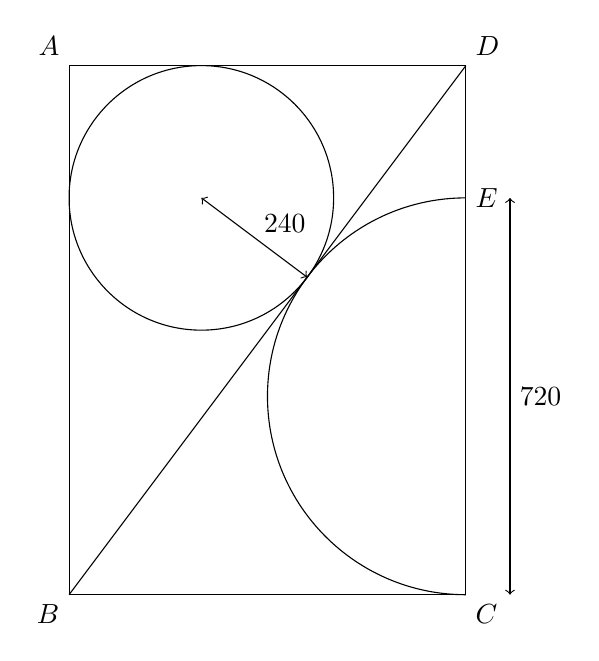
\begin{tikzpicture}[scale=0.7]
            \coordinate[label=above left:$A$] (A) at (0, 9.6);
            \coordinate[label=below left:$B$] (B) at (0, 0);
            \coordinate[label=below right:$C$] (C) at (7.2, 0);
            \coordinate[label=above right:$D$] (D) at (7.2, 9.6);
            \coordinate[label=right:$E$] (E) at (7.2, 7.2);

            \draw (A) -- (B) -- (C) -- (D) -- (A);
            \draw (B) -- (D);

            \draw (2.4, 7.2) circle[radius=2.4];
            \draw (7.2, 7.2) arc(90:270:3.6);

            \draw[<->] (2.4, 7.2) -- (4.32, 5.76);
            \draw[<->] (8, 0) -- (8, 7.2);

            \node[anchor=west] at (8, 3.6) {720};
            \node[anchor=south west] at (3.36, 6.4) {240};
        \end{tikzpicture}
    \end{center}
\end{enumerate}